\documentclass[a4paper,10pt]{article}

\usepackage{amsmath}
\usepackage{amsfonts}
\usepackage{amsthm}
\usepackage{fourier}
\usepackage{multirow}
\usepackage{tikz}
\usepackage[a4paper, margin=.5in]{geometry}

\usetikzlibrary{arrows.meta, positioning}
\newtheorem{assumption}{Assumption}
\newtheorem{lemma}{Lemma}
\newtheorem{remark}{Remark}

\title{}
\date{}
\author{}

\begin{document}
\maketitle
\section{Introduction}

Advanced cancer stages are inherently more difficult to treat than earlier ones. As patients progress through successive lines of therapy, they accumulate treatment related side effects including toxicities and, in some cases, irreversible organ damage, progressively narrowing their therapeutic options. Metastatic cancer represents one of the most challenging of these advanced stages, characterized by the systemic spread of tumor cells throughout the body. In this setting, patients frequently relapse, mortality rates remain high, and clinical management must navigate the competing risks of disease progression and cumulative treatment burden. The biological complexity of metastasis further complicates the development of effective therapies: strict eligibility criteria are required to manage patient heterogeneity in clinical trials, early detection of progression is challenging, and the competing risks of toxicity and disease activity increase the probability of trial failure.

Metastatic breast cancer (mBC) is one of the most studied instances of this challenge and an area of particularly active therapeutic development. Breast cancer is broadly classified according to its hormonal receptor profile, with the three main subtypes being HR+/HER2-, HER2+, and triple-negative (TN). These subtypes differ substantially in their biology, prognosis, and available treatment options, with the triple-negative subtype being the most aggressive and associated with the poorest overall survival. The HR+/HER2- subtype, being the most frequent, is particularly well characterized. However, these population level figures mask a wide heterogeneity in individual outcomes, driven by differences in tumor biology, patient characteristics, and the cumulative pressure of prior treatments. This variability makes predicting individual patient trajectories and selecting the most appropriate treatment strategy a genuinely difficult clinical problem.

\paragraph{The Structure of Treatment in mBC}
Treatment for metastatic breast cancer is organized into sequential lines of therapy, each separated by a progression event defined as the appearance of new metastatic sites or the measurable growth of existing lesions. Within each line, treatment decisions are guided by subtype specific standards of care, meaning they follow population level recommendations rather than being tailored to the individual patient. As patients progress through successive lines, these guidelines become increasingly insufficient: the patient's profile diverges from the population on which the recommendations were built, and the space of reasonable therapeutic options grows harder to navigate. Studying the full combinatorial space of possible treatment sequences would in principle require a very large number of prospective clinical trials, each demanding substantial resources and each subject to the enrollment and design difficulties described above. Real world medical records offer a complementary source of evidence: they capture the full longitudinal treatment trajectory of patients as it unfolds in clinical practice, at a scale and with a breadth of representation that prospective trials cannot match.

\paragraph{The Need for Causal Inference}
However, real world data cannot be used naively to compare treatment strategies. Because treatment assignment is not randomized, it is systematically driven by patient characteristics: sicker patients or those with more aggressive disease may be more or less likely to receive certain treatments, creating systematic differences between treatment arms that have nothing to do with the treatment itself. This phenomenon, known as confounding, means that a naive comparison of outcomes across treatment arms, for instance by fitting a Cox proportional hazards model to each arm separately, risks attributing to the treatment what is in fact due to differences in the patient population. Randomized controlled trials eliminate confounding by design, breaking the link between patient characteristics and treatment assignment. In observational settings, the field of causal inference provides a principled framework for recovering unconfounded treatment effect estimates from non-randomized data, under explicit and testable assumptions. Within this framework, the target trial emulation methodology offers a structured approach to using real world data to answer causal questions about treatment strategies, by explicitly defining the hypothetical trial one aims to emulate and applying appropriate methods to adjust for confounding.

\paragraph{Survival Analysis as the Outcome Framework}
A natural and clinically meaningful way to evaluate treatment strategies in this setting is through survival analysis, which models the time from a given starting point to an event of interest, typically death or disease progression. Classical approaches such as the Cox proportional hazards model have long been the reference in this domain, offering interpretable estimates of treatment effects under the assumption that the hazard ratio between groups remains constant over time. However, in the metastatic setting where patient trajectories are longitudinal, dynamic, and shaped by a sequence of treatments and progression events, static survival models have important limitations. They cannot naturally incorporate time varying covariates or the evolving state of the patient across treatment lines, potentially missing important prognostic information. More flexible approaches, including those based on neural networks, have been developed to address these limitations and have been shown to outperform classical models in several settings. Embedding survival analysis within a causal inference framework further allows one to move from association to causation, estimating not simply which patients tend to survive longer but what survival benefit a given patient would derive from a specific treatment strategy relative to an alternative.

\section{Problem Formulation and Causal Structure}

\subsection{Patient Representation}

Each patient is represented by three sequences: $X_{1:L}$ the patient state sequence, $A_{1:L}$ the treatment sequence, and $Y_{1:L} := (P, O)_{1:L}$ the survival outcome sequence, where $P_k$ and $O_k$ denote the progression-free survival and overall survival at line $k$, respectively. At each treatment line $k$, the tuple $(X_k, A_k, P_k, O_k)$ represents the patient's clinical state at the onset of line $k$, the treatment administered during that line, and the resulting survival outcomes.

\subsection{Treatment Line Definition}

A treatment line is defined recursively from the patient's history. The first line begins when the patient initiates treatment for metastatic disease. A line ends upon disease progression, defined as the appearance of new metastases or growth of existing ones. The subsequent line begins at the onset of the next treatment. The period between the end of one line and the start of the next is referred to as the \textit{buffer time}.



\subsection{Causal Structure and Generative Process}

In observational data, treatment assignment $A_k$ is not random. It depends on the patient's clinical state $X_k$ and on the history of previous treatments and outcomes. We denote by
\begin{equation}
    H_k^- := (X_{1:k-1},\, A_{1:k-1},\, P_{1:k-1})
\end{equation}
the history strictly prior to line $k$, and by
\begin{equation}
    H_k := H_k^- \cup \{X_k\} = (X_{1:k},\, A_{1:k-1},\, P_{1:k-1})
\end{equation}
the full information available to the treating physician at the decision point of line $k$. This dependency creates confounding: a model that naively associates treatments with outcomes reflects physician selection patterns rather than true treatment effects.

To account for this, we adopt a sequential causal structure that mirrors the clinical decision process. The joint distribution over patient trajectories factorizes as
\begin{equation}
    P(X_{1:L}, A_{1:L}, P_{1:L}, O_{1:L}) 
    = \prod_{k=1}^{L} 
    \underbrace{P(X_k \mid H_k^-)}_{\text{state transition}} \;
    \underbrace{P(A_k \mid H_k)}_{\text{treatment assignment}} \;
    \underbrace{P(P_k \mid H_k, A_k)}_{\text{progression-free survival}} \;
    \underbrace{P(O_k \mid H_k, A_k)}_{\text{overall survival}}
    \label{eq:factorization}
\end{equation}
with the convention $X_0 = A_0 = P_0 = \emptyset$, and where factors at line $k$ are defined only on the event that the patient is alive at its onset (i.e., the patient survived line $k-1$). Patients who die during line $k$ contribute no further terms beyond that line. This factorization encodes the temporal ordering of the decision process and forms the structural backbone of our model. 
% Rather than proposing a new causal inference method, we leverage this structure to build a treatment recommendation model that accounts for time-varying confounding across lines of therapy.

A central feature of this structure is the dual role of progression-free survival $P_k$: it is simultaneously an outcome of line $k$ and a determinant of the next patient state $X_{k+1}$. Clinically, progression is the event that triggers the transition to the next line of therapy and redefines the patient's disease status. This is precisely the setting in which static causal adjustment fails and a sequential approach becomes necessary.

\begin{figure}[h]
\centering
\scalebox{0.7}{
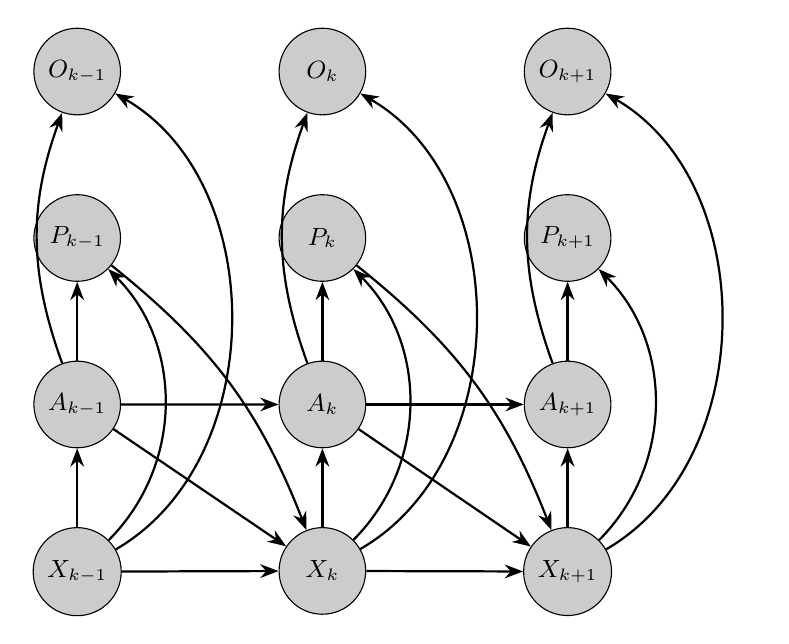
\begin{tikzpicture}[
    node distance=1.0cm and 2cm,
    arr/.style={-{Stealth}, thick},
    every node/.style={circle, draw, fill=gray!40, minimum size=1.1cm, font=\small},
]

    \node (O1) {$O_{k-1}$};
    \node[right=of O1] (O2) {$O_{k}$};
    \node[right=of O2] (O3) {$O_{k+1}$};

    \node[below=of O1] (P1) {$P_{k-1}$};
    \node[below=of O2] (P2) {$P_{k}$};
    \node[below=of O3] (P3) {$P_{k+1}$};

    \node[below=of P1] (A1) {$A_{k-1}$};
    \node[below=of P2] (A2) {$A_{k}$};
    \node[below=of P3] (A3) {$A_{k+1}$};

    \node[below=of A1] (X1) {$X_{k-1}$};
    \node[below=of A2] (X2) {$X_{k}$};
    \node[below=of A3] (X3) {$X_{k+1}$};

    \draw[arr] (X1) -- (A1);
    \draw[arr] (A1) -- (P1);
    \draw[arr] (A1) to[bend left=20] (O1);
    \draw[arr] (X1) to[bend right=45] (P1);
    \draw[arr] (X1) to[bend right=60] (O1);

    \draw[arr] (X2) -- (A2);
    \draw[arr] (A2) -- (P2);
    \draw[arr] (A2) to[bend left=20] (O2);
    \draw[arr] (X2) to[bend right=45] (P2);
    \draw[arr] (X2) to[bend right=60] (O2);

    \draw[arr] (X3) -- (A3);
    \draw[arr] (A3) -- (P3);
    \draw[arr] (A3) to[bend left=20] (O3);
    \draw[arr] (X3) to[bend right=45] (P3);
    \draw[arr] (X3) to[bend right=60] (O3);

    \draw[arr] (X1) -- (X2);
    \draw[arr] (X2) -- (X3);

    \draw[arr] (A1) -- (A2);
    \draw[arr] (A2) -- (A3);

    \draw[arr] (A1) -- (X2);
    \draw[arr] (A2) -- (X3);

    \draw[arr] (P1) to[bend left=15] (X2);
    \draw[arr] (P2) to[bend left=15] (X3);

\end{tikzpicture}
}
\caption{Sequential causal structure over treatment lines. $X_k$ is the patient state, $A_k$ the treatment, $P_k$ the progression-free survival, and $O_k$ the overall survival at line $k$. $O_k$ is a terminal node; $P_k$ feeds into the next state as progression triggers the next treatment line.}
\label{fig:dag}
\end{figure}

Figure~\ref{fig:dag} presents the sequential causal structure underlying our model. At each treatment line $k$, the patient state $X_k$ encodes the clinical information available at the onset of the line. The treating physician selects treatment $A_k$ based on $X_k$, but also explicitly conditions on the previous treatment $A_{k-1}$. \textcolor{red}{This reflects the clinical reality that treatment sequencing in oncology follows protocols and avoids repeating failed regimens}. Both $X_k$ and $A_k$ causally influence the two outcome nodes: the progression-free survival $P_k$ and the overall survival $O_k$. Crucially, $O_k$ is a terminal node: death is an absorbing state and carries no outgoing edges. In contrast, $P_k$ feeds into the next patient state $X_{k+1}$ via the edge $P_k \rightarrow X_{k+1}$, since progression is the clinical event that triggers the onset of the next treatment line and redefines the patient's disease status. The state transition $X_k \rightarrow X_{k+1}$ additionally depends on the administered treatment $A_k$, encoding the direct biological effect of treatment on disease evolution. This structure mirrors the sequential decision process a clinician follows and provides the causal backbone for our treatment recommendation model.

\subsection{Causal Estimand}
\label{sec:estimand}

We now formalize the quantity of interest and how it articulates witht the goal of treatment recommendation. At the onset of line $k$, the clinician faces a choice among treatments $a \in \mathcal{A}$, and the relevant question is what would the patient's survival be if, contrary to the observed decision, treatment $a$ were administered? Using the potential outcomes notation, let $O_k(a)$ denote the potential overall survival time at line $k$ under treatment $a$, and $P_k(a)$ the potential progression-free survival. Both are defined for every treatment $a \in \mathcal{A}$, regardless of which treatment was actually observed.

The causal estimand of interest is the conditional potential outcome distribution at line $k$, given the observed patient history $H_k$:
\begin{equation}
    S_a(t \mid H_k) := \mathbb{P}\big(O_k(a) > t \mid H_k\big), \qquad t \in \{1, \ldots, T\},\; a \in \mathcal{A}.
    \label{eq:estimand}
\end{equation}
This is the counterfactual overall survival curve at line $k$ under treatment $a$, conditional on everything known about the patient up to the decision point. Treatment recommendation then reduces to comparing $S_a(t \mid H_k)$ across candidate treatments via a scalar summary, for which we use the restricted mean survival time
\begin{align}
    RMST_a(\tau) = \frac{1}{\tau} \int_{0}^{\tau} S_a(t \mid H_k)\  dt
\end{align}

\paragraph{Scope of the intervention.}
The estimand in Equation~\ref{eq:estimand} defines $O_k(a)$ as the potential overall survival time under a \emph{static single-line intervention}: we intervene on $A_k$ only, setting it to $a$, and let the subsequent treatment sequence $A_{k+1:L}$ follow its natural distribution under the observed clinical policy encoded in Equation~\ref{eq:factorization}. Formally, $S_a(t \mid H_k) = \mathbb{P}(O_k(a) > t \mid H_k)$ identifies, under Consistency, Positivity and Sequential Ignorability, from the observational conditional $\mathbb{P}(O_k > t \mid H_k, A_k = a)$ in which the future treatments $A_{k+1:L}$ are \emph{marginalized} rather than fixed. Two consequences of this definition deserve emphasis. First, the estimated effect of setting $A_k = a$ decomposes into a direct pharmacological component and an indirect component mediated by the distribution of subsequent treatments that a line-$k$ decision of $a$ induces. We do not attempt to separate these two channels: isolating the controlled direct effect of $A_k$ on $O_k$ would require sequential ignorability at every future line rather than only at line $k$, together with an explicit model of the state-transition kernel $\mathbb{P}(X_{k+1} \mid H_k, A_k, P_k)$ under every candidate $a$, and a simulator that composes these kernels forward. Because future treatments $A_{k+1:L}$ are descendants of $A_k$ in the causal graph of Figure~\ref{fig:dag} rather than common causes of $A_k$ and $O_k$, the inclusion of the mediated channel does not constitute confounding: the estimator targets the \emph{total} effect of setting $A_k = a$, of which the indirect pathway through future care is a legitimate component. Second, and more importantly, this composite effect is precisely the quantity that maps onto the clinical decision the model is designed to support. At the onset of line $k$, the clinician commits only to $A_k$; the decisions at lines $k+1, k+2, \ldots$ will be made later, by the same clinical system that generated the training data, on the basis of the patient's future state. The decision-relevant question is therefore not ``what is the effect of $a$ on survival in isolation from all downstream care?''--a quantity no realizable intervention can produce--but ``what survival trajectory follows from choosing $a$ now, given that subsequent care will unfold as it normally does for patients like this one?'' Our estimand answers the second question, and the validity of the resulting recommendation rests on the deployment-time future-treatment policy remaining close to the one observed in the training data.

\paragraph{From single-line recommendation to sequential optimization.}
The framework developed here is deliberately restricted to single-line recommendation and does not claim to produce a globally optimal treatment sequence. Chaining locally optimal line-by-line recommendations does not in general recover the optimal regime: the choice at line $k$ alters the state distribution $\mathbb{P}(X_{k+1} \mid H_k, A_k, P_k)$, and hence the efficacy of the options available at every subsequent line. A treatment that is suboptimal at line $k$ in the sense of equation~\ref{eq:estimand} may nonetheless lead the patient into a state in which the remaining lines are substantially more effective, and the reverse situation is equally possible. Formalizing this trade-off requires moving from a single-line estimand to a dynamic treatment regime: one seeks a policy $\pi^{*} : H_k \mapsto \mathcal{A}$ maximizing a cumulative objective such as total RMST over the remaining horizon, which can be obtained by backward induction on the line index (Q-learning, G-estimation of structural nested mean models) or, when the state space is richer, by off-policy reinforcement learning over the full patient trajectory. Both approaches require strictly stronger identifying assumptions--sequential ignorability at every line rather than only at the decision point of interest---and additional modeling components such as an explicit state-transition model under each candidate treatment so that counterfactual trajectories can be simulated forward. The architecture introduced in Section~\ref{sec:model-overview} already provides several of the necessary ingredients: a shared history encoder, per-treatment outcome heads, and progression heads that summarize treatment response. Extending it to a full sequential policy optimizer is a natural direction for future work and is discussed in Section~\textcolor{red}{[discussion]}.

\subsection{Identifiability}

Estimating the effect of a treatment sequence from observational data requires that the interventional distributions of interest be identifiable from the observed data distribution. In the sequential setting, this relies on three standard assumptions.

\begin{assumption}[Consistency]
The observed outcome for a patient who received treatment $A_k = a$ is equal to the potential outcome under treatment $a$:
\begin{equation}
    A_k = a \implies O_k = O_k(a), \quad P_k = P_k(a)
\end{equation}
This assumption states that there are no multiple versions of a treatment a patient receiving treatment $a$ experiences exactly the outcome that would be expected under treatment $a$. In our setting, this is reasonable as treatment lines correspond to well-defined therapeutic regimens with no ambiguity about the expected outcome.
\end{assumption}

\begin{assumption}[Positivity]
For all treatment lines $k$ and all treatments $a \in \mathcal{A}$, the probability of receiving treatment $a$ is bounded away from zero for any patient history with positive support:
\begin{equation}
    P(X_{1:k}, A_{1:k-1}, P_{1:k-1}) > 0 \implies 
    P(A_k = a \mid X_{1:k}, A_{1:k-1}, P_{1:k-1}) > 0
\end{equation}
This ensures that every treatment option is observed across the patient population, 
allowing its effect to be estimated. \textcolor{red}{In practice, positivity may be violated for rare 
treatments or highly specific patient subgroups. This will be explored in the limitations of the model}
\end{assumption}

\begin{assumption}[Sequential Ignorability]
Given the observed patient history, treatment assignment at each line is independent of the potential outcomes:
\begin{equation}
    A_k \perp\!\!\!\perp \{O_k(a), P_k(a)\}_{a \in \mathcal{A}} 
    \mid X_{1:k}, A_{1:k-1}, P_{1:k-1}
\end{equation}
This is the key identifying assumption. It states that all confounders of the treatment decision are captured in the observed patient history $(X_{1:k}, A_{1:k-1}, P_{1:k-1})$, so that no unmeasured variable simultaneously influences treatment choice and outcomes. Clinically, this holds to the extent that physician decisions are driven by the recorded clinical state. While this assumption is untestable from observational data alone, it is standard in the causal inference literature for sequential treatment settings and is supported by the richness of the clinical variables available in our dataset.
\end{assumption}

\textcolor{red}{Here i will put the theorem (easy) and prove it in the appendix}

\begin{lemma}[Identifiability]
    Under Assumption 2 and 3 the counterfactual survival is identifiable. 
\end{lemma}

\section{Model}

\begin{figure}
    \centering
    \includegraphics[width=.6\textwidth]{model_architecture_small.drawio.pdf}
    \label{fig:modelarchi}
    \caption{Model architecture of the counterfactual survival prediction model \textcolor{red}{First draft figure requires legend and probably color coding of the blocks to distinguish prediction blocks from model ones, \warning there is a typo the heads should have O as superscript \warning}}
\end{figure}

\subsection{Overview}
\label{sec:model-overview}

Our goal is to recommend for a given patient with known history $H_k$ at the onset of line $k$ the treatment $a \in \mathcal{A}$ that maximizes the RMST at an arbitrarily chosen $\tau$. 
We adopt a \emph{static single-step} recommendation regime: given a patient whose observed history $H_k$ is available at a chosen decision point $k$, the model recommends a treatment for line $k$ only. We do not simulate future lines, nor do we optimize over a multi-step strategy $(a_k, a_{k+1}, \ldots)$. 

This task doesn't require modeling the whole data generation process but only requires modeling $P(O_k \mid H_k, A_k=a)$ for each candidate treatment $a$.
The architecture reflects this target directly. It consists of three components:
\begin{itemize}
    \item[i.] A shared history encoder $\phi$ that compresses $H_k$ into a fixed-size vector $h_k$
    \item[ii.] A set of progression heads  $\{f^P_a : a \in \mathcal{A}\}$, estimating the conditional distribution of $P_k$ given $h_k$
    \item[iii.] A set of overall survival heads $\{f^O_a : a \in \mathcal{A}\}$ per treatment, estimating the conditional distribution of $O_k$ given $h_k$. 
\end{itemize}
The one head per treatment \textcolor{red}{(Shalit)} design mirrors the potential outcomes framework: each head corresponds to a distinct counterfactual outcome model, and treatment is not passed as an input feature but selects which head is evaluated. Both sets of heads use a discrete-time hazard parametrization. 
The progression heads are used as an auxiliary multitask target, motivated by two observations about the role of progression in the causal structure of the problem. First, the latent factors that drive disease progression (tumor aggressiveness, treatment resistance and underlying patient frailty) overlap with those that drive mortality. Therefore, training the encoder to predict progression shapes the shared representation $h_k$ to capture features that are also prognostic for overall survival, improving the quality of the overall survival predictions used in the recommendation criterion. Second, progression at a past line $j<k$ is a proxy of the patient's response to the treatment $A_j$ administered at that line. An early progression signals that the chosen treatment family was ineffective for this patient, which is informative for selecting subsequent treatments for example by pivoting to a different mechanism of action. Carrying a learned progression representation forward through the encoder makes this treatment-response history available to the recommendation at line $k$.

\noindent \textcolor{red}{\warning This is starting to become tricky because passing precictions recursively is different from passing a value, adding this mechanism introduces the transition probability - worth specifying better to avoid confusion: Am i recommending at a single time step or recommending on all the time steps. \warning}
\subsection{History Encoder \textcolor{red}{(not sure yet)} }

\label{sec:encoder}

The encoder $\phi$ maps the patient history $H_k$ to a fixed-size representation $h_k \in \mathbb{R}^d$. At each line $j \leq k$, the input token is the concatenation
\begin{equation}
    u_j = [X_j,\, A_{j-1},\, \rho^P_{j-1}],
\end{equation}
with the convention $A_0 = \rho^P_0 = \emptyset$, and where $\rho^P_{j-1}$ is a summary of the progression risk at line $j-1$ derived from the progression head $f^P_{A_{j-1}}$. Concretely, $\rho^P_{j-1}$ is obtained by passing the history representation $h_{j-1}$ through the progression head indexed by the treatment administered at line $j-1$, yielding a discrete hazard vector over time bins. The sequence $u_{1:k}$ is then processed by a unidirectional LSTM:
\begin{equation}
    h_k = \text{LSTM}(u_{1:k}),
\end{equation}
where $h_k$ is the hidden state at the final step.

Two remarks on this design. First, feeding a predicted progression representation rather than the observed progression time carries the learned treatment-response signal forward through the encoder in a form that is well-defined regardless of censoring status at line $j-1$, and that is smooth in the prognostic information extracted by the progression head. Second, this creates a recurrent coupling between the encoder and the progression head: the encoder produces $h_{j-1}$, which the progression head uses to produce $\rho^P_{j-1}$, which in turn feeds the encoder at step $j$. This coupling is trained end-to-end via backpropagation through time. The encoder is shared across all treatments and across both outcome heads, providing a common patient representation on top of which the treatment-specific heads operate.

\subsection{Treatment-Specific Survival Heads}
\label{sec:survival-heads}

For each treatment $a \in \mathcal{A}$, the model maintains two dedicated heads: a progression head $f^P_a$ and an overall survival head $f^O_a$. Both are multilayer perceptrons that output a discrete hazard function over a fixed grid of time bins $\{1, \ldots, T\}$.
The heads $f^P_a$ and $f^O_a$ take $h_k$ as input and each outputs a vector of discrete hazards
\begin{equation}
    \hat{\lambda}^P_a(t \mid h_k) = \sigma\left( f^P_a(h_k)_t \right) \qquad
    \hat{\lambda}^O_a(t \mid h_k) = \sigma\left( f^O_a(h_k)_t \right)
    , \qquad t = 1, \ldots, T
\end{equation}
where $\sigma$ is the sigmoid function. The corresponding survival functions are
\begin{equation}
    \hat{S}^P_a(t \mid h_k) = \prod_{s=1}^{t} \left( 1 - \hat{\lambda}^P_a(s \mid h_k) \right) \qquad
    \hat{S}^O_a(t \mid h_k) = \prod_{s=1}^{t} \left( 1 - \hat{\lambda}^O_a(s \mid h_k) \right)
\end{equation}
estimating $P(P_k > t \mid H_k, A_k = a)$ and $P(O_k > t \mid H_k, A_k = a)$.

\subsection{Training Objective}
\label{sec:training}

Each patient contributes at each observed line $k$ a supervised signal to exactly one progression head and one overall survival head. The remaining heads receive no gradient from this patient at this line. This is the natural consequence of the potential-outcomes formulation.

Both heads are trained with the logistic hazard loss \textcolor{red}{Kvamme continuous and discrete time survival prediction}.

The logistic hazard loss is the discrete-time negative log-likelihood under right-censoring. Let time be discretized into bins $\{\tau_1, \ldots, \tau_T\}$, and for each patient $i$ let $t_i$ be the observed duration, $d_i \in \{0, 1\}$ the event indicator ($d_i = 1$ for an observed event, $d_i = 0$ for censoring), and $\kappa(t_i)$ the index of the bin containing $t_i$. Assuming independent censoring and that the event-time and censoring distributions share no parameters, the likelihood contribution of patient $i$ decomposes into a product over the hazards at each bin up to $\kappa(t_i)$:
\begin{equation}
    L_i = \hat{\lambda}(\tau_{\kappa(t_i)})^{d_i} \, [1 - \hat{\lambda}(\tau_{\kappa(t_i)})]^{1 - d_i} \prod_{j=1}^{\kappa(t_i) - 1} [1 - \hat{\lambda}(\tau_j)].
\end{equation}
Taking the negative log and summing over patients, the loss can be rewritten as a double sum over patients and time bins:
\begin{equation}
    \mathcal{L}_{surv}(t_i, \delta) = -\frac{1}{n} \sum_{i=1}^{n} \sum_{j=1}^{\kappa(t_i)} \Big( y_{ij} \log \hat{\lambda}(\tau_j \mid h_i) + (1 - y_{ij}) \log [1 - \hat{\lambda}(\tau_j \mid h_i)] \Big),
    \label{eq:logistic-hazard-loss}
\end{equation}
where $y_{ij} = \mathbf{1}\{j = \kappa(t_i),\, d_i = 1\}$ indicates whether patient $i$ experiences the event in bin $j$. This is exactly a binary cross-entropy over the discrete hazards: at each bin before the observed time the label is $0$ ("survived"), and at the terminal bin the label is $d_i$ (event) or $0$ (censored). This form is what the model optimizes in practice, implemented as a masked binary cross-entropy on the hazard output vector.

Summing over patients $i$, lines $k$, and the two heads yields the total objective
\begin{equation}
    \mathcal{L}_{\text{total}} = \sum_{i, k} \mathcal{L}_{surv}(O_{i,k}, \delta^O_{i,k}) + \mathcal{L}_{surv}(P_{i,k}, \delta^P_{i,k})
\end{equation}
where $P_{i,k}$ and $O_{i,k}$ are the observed progression and overall survival times for patient $i$ at line $k$, and $\delta^P_{i,k}, \delta^O_{i,k}$ are the associated event indicators. The encoder $\phi$ is updated jointly with all treatment-specific heads via standard backpropagation.

\subsection{Representation balancing}

Because treatment assignment is confounded by the patient history $H_k$, patients who received treatment $a$ are systematically different from those who received $a'$. Following the counterfactual regression framework of \textcolor{red}{[Shalit et al., 2017; Johansson et al., 2022]}, we address this by regularizing the encoder to produce representations whose distribution is approximately balanced across treatments. Concretely, let $\Phi_a := \{h_{i,k} : A_{i,k} = a\}$ denote the set of patient representations observed under treatment $a$ in a minibatch, and let $\text{IPM}(\Phi_a, \Phi_{a'})$ be an integral probability metric between the empirical distributions of $\Phi_a$ and $\Phi_{a'}$. The balancing term is

\begin{equation}
    \mathcal{L}_{\text{IPM}} = \sum_{a, a' \in \mathcal{A}} \text{IPM}(\Phi_a, \Phi_{a'}),
\end{equation}
and the full training objective becomes
\begin{equation}
    \mathcal{L} = \mathcal{L}_{\text{total}} + \alpha \, \mathcal{L}_{\text{IPM}},
\end{equation}

where $\alpha > 0$ controls the strength of the balancing regularizer. 
Minimizing $\mathcal{L}_{\text{IPM}}$ encourages the encoder to discard features of the patient history that are predictive of treatment assignment but not of outcome, so that the representation space on which the outcome heads operate is comparable across treatment arms. \textcolor{red}{link to the section where the result between different IPM measures is discussed.}

\subsection{Inference and Treatment Recommendation}
\label{sec:inference}

At inference time, for a patient with history encoded as $h_k$, the model evaluates each candidate treatment $a \in \mathcal{A}$ by computing the survival curve $\hat{S}^O_a(t \mid h_k)$ from the corresponding overall survival head. The curve is summarized by the restricted mean survival time up to a 

\begin{equation}
    \widehat{\text{RMST}}_a(\tau) = \sum_{t=1}^{T} \hat{S}^O_a(t \mid h_k),
\end{equation}
and the recommended treatment is obtained by comparing candidates pairwise via the estimand of Equation~\ref{eq:estimand} or, equivalently, by direct maximization:
\begin{equation}
    \hat{a}^*(\tau) = \arg\max_{a \in \mathcal{A}} \widehat{\text{RMST}}_a.
\end{equation}



\section{Data}

For each patient and each treatment line $k$ at which the patient is alive, we build a record containing the full medical history summarized up to the progression date of line $k-1$ (or, at $k=1$, up to the date of metastatic diagnosis), together with the treatment $A_k$ administered at line $k$. This record is the observational realization of the pair $(H_k, A_k)$ defined in Section~2. The associated outcomes are the observed progression-free survival $P_k$, measured from the first day of line $k$ to the next progression, and the overall survival $O_k$, measured from the first day of line $k$ to death or censoring. A patient alive at the onset of line $k$ contributes one record to the cohort at that line; patients who died during an earlier line contribute no further records.

This construction has two consequences for the modeling framework. First, the prediction target at line $k$ is survival measured from the first day of line $k$, conditional on the patient being alive at its onset. Second, the history $H_k$ explicitly incorporates all previous treatments $A_{1:k-1}$ and progression events $P_{1:k-1}$, so that the encoder of Section~\ref{sec:encoder} has access to the full sequence of past decisions and responses.


\section{Model Validation}

\subsection{Factual Prediction Quality}
\label{sec:factual-validation}

We first assess whether the model fits the observational data well, before turning to the harder question of counterfactual validity. At each treatment line $k$, every patient in the test set has an observed treatment $A_{i,k}$, an observed outcome $(O_{i,k}, \delta^O_{i,k})$, and a model prediction $\hat{S}^O_{A_{i,k}}(t \mid h_{i,k})$ produced by the head corresponding to the actually administered treatment. Factual prediction quality is evaluated by comparing this prediction against the observed survival outcome, using the time-dependent C-index, the integrated Brier score (IBS), and expected calibration error (ECE). Definitions and formulas for these metrics are deferred to Appendix~\textcolor{red}{It will be added in the appendix later}.

We compare our model against three external baselines and three ablations of our own architecture, allowing us to isolate the contribution of each design choice:

\begin{itemize}
    \item \textbf{Cox-Net PH} (per line, fitted independently). An Cox proportional hazards model with elastic net regularization fitted at each line $k$ on the patient state $X_k$ and treatment indicator $A_k$. This is the conventional clinical baseline.
    \item \textbf{DeepSurv (flat history) } \textcolor{red}{Deep learning based cox}. A multilayer perceptron applied per-line to the same flat feature vector $[X_k, A_k]$, trained with the partial likelihood loss. This isolates the value of nonlinear modeling without any sequential or causal structure.
    \item \textbf{SurvITE}. \textcolor{red}{More recent baselines that will probably be needed} 
    \item \textbf{TARNet (flat history)}. A treatment-specific-head architecture identical to ours but without the sequential encoder, the auxiliary progression head, and the IPM regularizer. This isolates the value of the head structure alone.
    \item \textbf{RSF}. A random survival forest model 
    \item \textbf{Ours}. The complete architecture described in Section~\ref{sec:model-overview}.
\end{itemize}

All models are trained on the same training split, evaluated on the same held-out test set, and metrics are reported with bootstrap 95\% confidence intervals over 10 resamples of the test set.

\begin{table}[h]
\centering
\begin{tabular}{clccc}
\hline
\textbf{Line} & \textbf{Model} & \textbf{C-index $\uparrow$} & \textbf{IBS $\downarrow$} & \textbf{ECE $\downarrow$} \\
\hline
\multirow{7}{*}{1}
 & Cox PH                  & 0.578 [0.570, 0.588] & 0.144 [0.142, 0.146] & 0.003 [0.003, 0.020] \\
 & DeepSurv                & 0.670 [0.660, 0.680] & 0.131 [0.127, 0.134] & 0.043 [0.031, 0.062] \\
 
 & RSF                     & \textcolor{red}{.} & \textcolor{red}{.} & \textcolor{red}{.} \\
 & \textbf{Ours}    & \textcolor{red}{.} & \textcolor{red}{.} & \textcolor{red}{.} \\
\hline
\multirow{7}{*}{2}
 & Cox PH                  & 0.558 [0.544, 0.570] & 0.139 [0.135, 0.142] & 0.005 [0.002, 0.019] \\
 & DeepSurv                & 0.652 [0.641, 0.662] & 0.129 [0.123, 0.134] & 0.072 [0.060, 0.086] \\
 & RSF                     & \textcolor{red}{.} & \textcolor{red}{.} & \textcolor{red}{.} \\
 & \textbf{Ours}    & \textcolor{red}{.} & \textcolor{red}{.} & \textcolor{red}{.} \\
\hline
\multirow{7}{*}{3}
 & Cox PH                  & 0.624 [0.612, 0.637] & 0.149 [0.145, 0.153] & 0.022 [0.012, 0.037] \\
 & DeepSurv                & 0.652 [0.641, 0.665] & 0.148 [0.141, 0.153] & 0.089 [0.077, 0.106] \\
 & RSF                     & \textcolor{red}{.} & \textcolor{red}{.} & \textcolor{red}{.} \\
 & \textbf{Ours}    & \textcolor{red}{.} & \textcolor{red}{.} & \textcolor{red}{.} \\
\hline
\multirow{7}{*}{4}
 & Cox PH                  & 0.478 [0.464, 0.499] & 0.177 [0.173, 0.181] & 0.005 [0.000, 0.028] \\
 & DeepSurv                & 0.627 [0.609, 0.643] & 0.182 [0.174, 0.190] & 0.156 [0.137, 0.175] \\
 & RSF                     & \textcolor{red}{.} & \textcolor{red}{.} & \textcolor{red}{.} \\
 & \textbf{Ours}    & \textcolor{red}{.} & \textcolor{red}{.} & \textcolor{red}{.} \\
\hline
\end{tabular}
\caption{Factual prediction quality by treatment line. Values are mean [95\% CI] over bootstrap resamples of the test set.}
\label{tab:factual-perline}
\end{table}

Table~\ref{tab:factual-perline} reports the C-index, IBS and ECE as a function of treatment line for each model. \textcolor{red}{[One sentence on the trend: e.g., performance is highest at line 1 where the patient population is most homogeneous, and decreases at later lines as data become sparser and patient heterogeneity increases. The relative ordering of models is consistent across lines / changes at later lines, suggesting that ...].}

\begin{figure}[h]
\centering
\textcolor{red}{[Figure: two side-by-side panels. Left: C-index vs treatment line, one curve per model with shaded 95\% CI bands. Right: IBS vs treatment line, same layout. x-axis: line index $k = 1, \ldots, K_{\max}$. Vertical dashed line marking the line beyond which sample sizes drop below the reliability threshold, if relevant.]}
\caption{Factual prediction quality as a function of treatment line}
\label{fig:factual-perline}
\end{figure}

\paragraph{Calibration.} The C-index and IBS summarize discrimination and overall accuracy but do not directly assess whether predicted survival probabilities are well-aligned with observed frequencies. Figure~\ref{fig:calibration} shows calibration curves at evaluation horizons of $t = 6, 12, 18, 24$ months, stratified by treatment line. Calibration curves at later lines ($k \geq 3$) lie close to the diagonal across the full range of predicted survival. At line~1, however, we observe a systematic upward shift: predicted survival underestimates observed survival with line~2 exhibiting a smaller but qualitatively similar offset. The shift consistent across the four evaluation horizons, indicating a score-level offset.

We attribute this pattern to a distribution-shift effect intrinsic to the shared-encoder design. Patients at line~1 form a healthier subpopulation than those at later lines, since reaching line~$k$ requires having progressed through lines $1, \ldots, k-1$. Because the encoder is shared across all lines, the learned hazard scale reflects an average across line-specific subpopulations and is too pessimistic when applied to the healthier line-1 cohort. The effect attenuates at later lines as their patient distributions move closer to the pooled mean, which matches the gradient observed in Figure~\ref{fig:calibration}.

Well-calibrated absolute probabilities are required for downstream uses of the model, including RMST estimation and clinical reporting. We therefore apply a post-hoc per-line, per-arm isotonic recalibration on a held-out fold; calibration curves after recalibration are reported in \textcolor{red}{isotonic regression appendix}. The recalibration is monotone by construction and therefore preserves all rank-based metrics like C-index.

\begin{figure}[h]
\centering
\includegraphics[width=\linewidth]{figs/output.png}
\caption{Calibration of the full model at evaluation horizons $t \in \{6, 12, 18, 24\}$ months, stratified by treatment line. Each point is a \textcolor{red}{ventile (code dependant)} of predicted survival on the test set; the $y$-coordinate is the observed Kaplan-Meier estimate within the decile. The diagonal corresponds to perfect calibration.}

% Line~1 exhibits a systematic underestimation of survival; calibration improves with line index, reflecting reduced distribution shift from the pooled training population. Curves before post-hoc recalibration.}

\label{fig:calibration}
\end{figure}

% \paragraph{Summary.} \textcolor{red}{[Two-three sentences. The model achieves [headline performance]. The ablation pattern shows that [which components matter most]. Calibration confirms that probabilistic outputs are reliable enough to support the recommendation analysis in Section~\ref{sec:recommendation}.]}




\section{Counterfactual validation}



% =======================================================================================
% ----------------------------- Possible appendix ---------------------------------------
% =======================================================================================

% \paragraph{Brier score.} The Brier score measures the mean squared error between the predicted survival probability and the observed survival status at a fixed evaluation time $t$. For right-censored data, we use the inverse-probability-of-censoring weighted (IPCW) estimator of \textcolor{red}{[Graf et al., 1999]}:
% \begin{equation}
%     \widehat{\text{BS}}(t) = \frac{1}{n} \sum_{i=1}^{n} \left[ \frac{\hat{S}^O_{A_{i,k}}(t \mid h_{i,k})^2 \, \mathbf{1}\{O_{i,k} \leq t,\, \delta^O_{i,k} = 1\}}{\hat{G}(O_{i,k})} + \frac{(1 - \hat{S}^O_{A_{i,k}}(t \mid h_{i,k}))^2 \, \mathbf{1}\{O_{i,k} > t\}}{\hat{G}(t)} \right],
% \end{equation}
% where $\hat{G}$ is the Kaplan-Meier estimator of the censoring distribution. Lower is better. Reporting the Brier score across a grid of evaluation times $t$ yields a curve that captures prediction quality over the full follow-up horizon; we also report the integrated Brier score (IBS) as a single summary.

% \paragraph{Time-dependent concordance index.} The C-index evaluates discriminative performance: the proportion of comparable patient pairs whose predicted risk ordering agrees with the observed event ordering. We use the time-dependent variant of \textcolor{red}{[Antolini et al., 2005]}, which accounts for the fact that risk rankings can change over time in non-proportional-hazard models:
% \begin{equation}
%     \widehat{C}^{\text{td}} = \frac{\sum_{i,j} \mathbf{1}\{O_{i,k} < O_{j,k},\, \delta^O_{i,k} = 1\} \cdot \mathbf{1}\{\hat{S}^O_{A_{i,k}}(O_{i,k} \mid h_{i,k}) < \hat{S}^O_{A_{j,k}}(O_{i,k} \mid h_{j,k})\}}{\sum_{i,j} \mathbf{1}\{O_{i,k} < O_{j,k},\, \delta^O_{i,k} = 1\}}.
% \end{equation}
% A value of $0.5$ corresponds to random ordering, and $1.0$ to perfect concordance.

% \paragraph{Calibration curves.} The Brier score and C-index are summary statistics; calibration curves visualize whether predicted survival probabilities are well-aligned with observed frequencies across the risk distribution. At a fixed evaluation time $t$, patients are stratified into deciles of predicted survival $\hat{S}^O_{A_{i,k}}(t \mid h_{i,k})$, and within each decile we compare the mean predicted survival to the Kaplan-Meier estimate of the observed survival probability. A perfectly calibrated model lies on the diagonal; deviations above or below indicate systematic over- or under-prediction.

% All three metrics are computed on a held-out test set, separately at each treatment line $k$ and pooled across lines, to evaluate whether prediction quality is uniform across decision points or degrades at later lines where data are sparser.


% \section{Proof of the Sequential Factorization}
% \label{app:factorization-proof}

% \begin{lemma}[Sequential factorization]
% \label{lem:factorization}
% Let $(X_{1:L}, A_{1:L}, P_{1:L}, O_{1:L})$ denote a patient trajectory whose joint distribution is Markov with respect to the directed acyclic graph of Figure~\ref{fig:dag}. Then, on the event that the patient is alive at the onset of line $k$, the joint distribution factorizes as
% \begin{equation}
%     P(X_{1:L}, A_{1:L}, P_{1:L}, O_{1:L}) 
%     = \prod_{k=1}^{L} 
%     P(X_k \mid H_k^-) \,
%     P(A_k \mid H_k) \,
%     P(P_k \mid H_k, A_k) \,
%     P(O_k \mid H_k, A_k, P_k),
% \end{equation}
% where $H_k^- := (X_{1:k-1}, A_{1:k-1}, P_{1:k-1})$ and $H_k := H_k^- \cup \{X_k\}$, with the convention $X_0 = A_0 = P_0 = \emptyset$.
% \end{lemma}

% \begin{proof}
% The proof proceeds in two steps: a chain-rule expansion that holds for any joint distribution, followed by an application of the local Markov property of the DAG to simplify each factor.

% \paragraph{Step 1: Chain rule.}
% Order the variables according to the temporal structure of the decision process:
% \begin{equation}
%     X_1, A_1, P_1, O_1, \; X_2, A_2, P_2, O_2, \; \ldots, \; X_L, A_L, P_L, O_L.
% \end{equation}
% For each $k \in \{1, \ldots, L\}$, denote by $\mathcal{F}_k := (X_{1:k-1}, A_{1:k-1}, P_{1:k-1}, O_{1:k-1})$ the set of all variables preceding $X_k$ in this ordering. Applying the chain rule of probability yields
% \begin{align}
%     P(X_{1:L}, A_{1:L}, P_{1:L}, O_{1:L}) 
%     = \prod_{k=1}^{L} \Big[ 
%     & P(X_k \mid \mathcal{F}_k) \, \nonumber \\
%     & P(A_k \mid \mathcal{F}_k, X_k) \, \nonumber \\
%     & P(P_k \mid \mathcal{F}_k, X_k, A_k) \, \nonumber \\
%     & P(O_k \mid \mathcal{F}_k, X_k, A_k, P_k) 
%     \Big].
%     \label{eq:chain-rule}
% \end{align}
% This expansion is purely algebraic and holds for any joint distribution, without any independence assumption.

% \paragraph{Step 2: Simplification via the local Markov property.}
% The local Markov property states that, conditional on its parents in the DAG, each node is independent of all its non-descendants. We apply this property to each of the four factors above.

% \emph{State transition.} The node $X_k$ has parents $\{X_{k-1}, A_{k-1}, P_{k-1}\}$ in the DAG. All variables in $\mathcal{F}_k$ are non-descendants of $X_k$ (they precede it in the temporal ordering and the DAG is acyclic). By the local Markov property,
% \begin{equation}
%     P(X_k \mid \mathcal{F}_k) = P(X_k \mid X_{k-1}, A_{k-1}, P_{k-1}) = P(X_k \mid H_k^-),
% \end{equation}
% where the last equality holds because conditioning on the superset $H_k^- \supseteq \{X_{k-1}, A_{k-1}, P_{k-1}\}$ of non-descendants of $X_k$ leaves the conditional distribution unchanged.

% \emph{Treatment assignment.} The node $A_k$ has parents $\{X_k, A_{k-1}\}$ in the DAG. The conditioning set $(\mathcal{F}_k, X_k) = H_k \cup O_{1:k-1}$ consists of non-descendants of $A_k$: $H_k$ contains only variables from earlier lines and $X_k$ itself, while $O_{1:k-1}$ are terminal nodes from earlier lines, which by construction have no outgoing edges (death is an absorbing state) and are therefore non-descendants of $A_k$. The local Markov property gives
% \begin{equation}
%     P(A_k \mid \mathcal{F}_k, X_k) = P(A_k \mid X_k, A_{k-1}) = P(A_k \mid H_k).
% \end{equation}

% \emph{Progression-free survival.} The node $P_k$ has parents $\{X_k, A_k\}$ in the DAG. The conditioning set $(\mathcal{F}_k, X_k, A_k) = H_k \cup \{A_k\} \cup O_{1:k-1}$ again consists of non-descendants of $P_k$, by the same argument as above. Hence
% \begin{equation}
%     P(P_k \mid \mathcal{F}_k, X_k, A_k) = P(P_k \mid X_k, A_k) = P(P_k \mid H_k, A_k).
% \end{equation}

% \emph{Overall survival.} The node $O_k$ has parents $\{X_k, A_k, P_k\}$ in the DAG. The conditioning set $(\mathcal{F}_k, X_k, A_k, P_k)$ consists of non-descendants of $O_k$, since $O_k$ is terminal and therefore has no descendants at all. Applying the local Markov property,
% \begin{equation}
%     P(O_k \mid \mathcal{F}_k, X_k, A_k, P_k) = P(O_k \mid X_k, A_k, P_k) = P(O_k \mid H_k, A_k, P_k).
% \end{equation}

% \paragraph{Step 3: Conclusion.}
% Substituting the four simplified factors back into the chain-rule expansion~\eqref{eq:chain-rule} yields
% \begin{equation}
%     P(X_{1:L}, A_{1:L}, P_{1:L}, O_{1:L}) 
%     = \prod_{k=1}^{L} 
%     P(X_k \mid H_k^-) \,
%     P(A_k \mid H_k) \,
%     P(P_k \mid H_k, A_k) \,
%     P(O_k \mid H_k, A_k, P_k),
% \end{equation}
% which is the desired factorization. Note that the outcome variables $O_{1:k-1}$ from previous lines drop out of every factor: they are terminal in the DAG and therefore non-descendants of all variables at lines $k$ and beyond. Operationally, conditioning on the event that the patient is alive at the onset of line $k$ (i.e., $O_j > t_j$ for $j < k$) encodes all the information $O_{1:k-1}$ carries for surviving patients, so restricting the factorization to this event loses no information.
% \end{proof}

% a clarification maybe not necessary
% \begin{remark}[Minimal vs.\ convenient sufficient sets]
% The local Markov property would allow each factor to be written in terms of its \emph{minimal} parent set (e.g., $P(A_k \mid X_k, A_{k-1})$ rather than $P(A_k \mid H_k)$). We deliberately write the factorization using the uniform conditioning set $H_k$ for two reasons. First, conditioning on a superset of the parents that consists of non-descendants leaves the conditional distribution unchanged, so no information is lost. Second, using $H_k$ throughout matches both the sequential ignorability assumption (Assumption 3), which is stated in terms of $H_k$, and the LSTM encoder $\phi(X_{1:k}, A_{1:k-1})$, which summarizes the full history rather than a minimal sufficient statistic. This uniformity simplifies the statement and proof of the identifiability result that follows.
% \end{remark}

\end{document}